%&pdflatex
\documentclass[11pt,onecolumn]{scrartcl}
\usepackage[utf8]{inputenc}
\usepackage{amsmath,amssymb,amsfonts,mathrsfs,amsthm}
\usepackage[top=2cm,bottom=3cm,left=2.5cm,right=2cm]{geometry}
\usepackage{amssymb}
\usepackage{listings}
\usepackage{array}
\usepackage{mathtools}
\usepackage{dsfont}
\usepackage{graphicx}
\usepackage{pdfpages}
\usepackage[textsize=footnotesize,color=green]{todonotes}
\usepackage{algorithm, algorithmic}
\usepackage{array}
\usepackage{bm}
\usepackage{tikz}
\usepackage{subfigure}
\usepackage[normalem]{ulem}

\newcommand{\bs}[1]{\boldsymbol{#1}}
\DeclareMathOperator{\diag}{diag}

\newcommand{\equaldef}{\stackrel{\mathrm{def}}{=}}

\newcommand{\tablab}[1]{\label{tab:#1}}
\newcommand{\tabref}[1]{Table~\ref{tab:#1}}

\newcommand{\theolab}[1]{\label{theo:#1}}
\newcommand{\theoref}[1]{\ref{theo:#1}}
\newcommand{\eqnlab}[1]{\label{eq:#1}}
\newcommand{\eqnref}[1]{\eqref{eq:#1}}
\newcommand{\seclab}[1]{\label{sec:#1}}
\newcommand{\secref}[1]{\ref{sec:#1}}
\newcommand{\lemlab}[1]{\label{lem:#1}}
\newcommand{\lemref}[1]{\ref{lem:#1}}

\newcommand{\mb}[1]{\mathbf{#1}}
\newcommand{\mbb}[1]{\mathbb{#1}}
\newcommand{\mc}[1]{\mathcal{#1}}
\newcommand{\nor}[1]{\left\| #1 \right\|}
\newcommand{\snor}[1]{\left| #1 \right|}
\newcommand{\LRp}[1]{\left( #1 \right)}
\newcommand{\LRs}[1]{\left[ #1 \right]}
\newcommand{\LRa}[1]{\left\langle #1 \right\rangle}
\newcommand{\LRc}[1]{\left\{ #1 \right\}}
\newcommand{\tanbui}[2]{\textcolor{blue}{\sout{#1}} \textcolor{red}{#2}}
\newcommand{\Grad} {\ensuremath{\nabla}}
\newcommand{\Div} {\ensuremath{\nabla\cdot}}
\newcommand{\Nel} {\ensuremath{{N^\text{el}}}}
\newcommand{\jump}[1] {\ensuremath{\LRs{\!\left[#1\right]\!}}}
\newcommand{\uh}{\widehat{u}}
\newcommand{\fnh}{\widehat{f}_n}
\renewcommand{\L}{L^2\LRp{\Omega}}
\newcommand{\pO}{\partial\Omega}
\newcommand{\Gh}{\Gamma_h}
\newcommand{\Gm}{\Gamma_{-}}
\newcommand{\Gp}{\Gamma_{+}}
\newcommand{\Go}{\Gamma_0}
\newcommand{\Oh}{\Omega_h}

\newcommand{\eval}[2][\right]{\relax
  \ifx#1\right\relax \left.\fi#2#1\rvert}

\def\etal{{\it et al.~}}

\newcommand{\vect}[1]{\ensuremath\boldsymbol{#1}}
\newcommand{\tensor}[1]{\underline{\vect{#1}}}
\newcommand{\del}{\Delta}
\newcommand{\grad}{\nabla}
\newcommand{\curl}{\grad \times}
\renewcommand{\div}{\grad \cdot}
\newcommand{\ip}[1]{\left\langle #1 \right\rangle}
\newcommand{\eip}[1]{a\left( #1 \right)}
\newcommand{\pd}[2]{\frac{\partial#1}{\partial#2}}
\newcommand{\pdd}[2]{\frac{\partial^2#1}{\partial#2^2}}

\newcommand{\circone}{\ding{192}}
\newcommand{\circtwo}{\ding{193}}
\newcommand{\circthree}{\ding{194}}
\newcommand{\circfour}{\ding{195}}
\newcommand{\circfive}{\ding{196}}

\def\arr#1#2#3#4{\left[
\begin{array}{cc}
#1 & #2\\
#3 & #4\\
\end{array}
\right]}
\def\vecttwo#1#2{\left[
\begin{array}{c}
#1\\
#2\\
\end{array}
\right]}
\def\vectthree#1#2#3{\left[
\begin{array}{c}
#1\\
#2\\
#3\\
\end{array}
\right]}
\def\vectfour#1#2#3#4{\left[
\begin{array}{c}
#1\\
#2\\
#3\\
#4\\
\end{array}
\right]}

\newtheorem{proposition}{Proposition}
\newtheorem{corollary}{Corollary}
\newtheorem{theorem}{Theorem}
\newtheorem{lemma}{Lemma}

\newcommand{\G} {\Gamma}
\newcommand{\Gin} {\Gamma_{in}}
\newcommand{\Gout} {\Gamma_{out}}

\newtheorem{remark}{Remark}

\author{Jesse Chan\textsuperscript{a}, Jay Gopalakrishnan\textsuperscript{b}, and Leszek Demkowicz\textsuperscript{a}}

%\title{$\epsilon$-explicit analysis of DPG for convection-dominated diffusion}
\title{Global effects in locally optimal DPG test functions for convection-diffusion problems}
\date{}
\begin{document}

\maketitle
\begin{center}
\textsuperscript{a} Institute for Computational Engineering and Sciences, \\University of Texas at Austin, \\Austin, TX 78712, USA\\
\end{center}

\begin{center}
\textsuperscript{b} Department of Mathematics\\Portland State University, \\
Portland, OR 97207, USA
%\textsuperscript{b} Facultad de Matem\'aticas, \\Pontificia Universidad Cat\'olica de Chile,\\
%Avenida Vicu\~na Mackenna 4860, Santiago, Chile
\end{center}

\tableofcontents

\section{Introduction to DPG}

The Discontinuous Petrov-Galerkin method was originally introduced by Demkowicz and Gopalakrishnan in 2008 method as a way to attain automatic inf-sup stability for any well-posed variational problem through the construction optimal test functions \cite{DPG2}.  The method was later shown to be equivalent to the minimum residual method applied to the operator residual corresponding to a variational formulation \cite{DPG2, ChanHeuerBui-ThanhDemkowicz12}.  

The derivation of the DPG method can be briefly summarized as follows: we are given a trial space $U$ and discrete trial space $U_h \subset U$, Hilbert test space $V$, and a well-posed variational problem: find $u_h\in U_h$  such that
\begin{align}
\label{variational}
&b(u_h,v) = l(v), \quad \forall v\in V, 
\end{align}
where $b(u,v)$ is a bilinear form and $l \in V'$. If we identify the variational operator $B: U\rightarrow V'$ such that $\LRa{Bu,v} \coloneqq b(u,v)$, we can write the above variational formulation as an operator equation in $V'$
\[
Bu_h = l.
\]
Seeking the minimization of the discrete residual $\frac{1}{2} \nor{Bu_h-l}^2_{V'}$, we arrive at the normal equations 
\[
\LRp{Bu_h-l,B\delta u}_{V'} = 0, \quad \forall \delta u \in U_h.  
\]
Since $V$ is Hilbert, we can introduce the Riesz map $R_V:V \rightarrow V'$, an isometric map such that $\LRa{R_V v,\cdot} = \LRp{v,\cdot}_V$. By taking the inverse of the Riesz map, we can transform the normal equations in $V'$ to a set of normal equations in $V$
\[
\LRp{R_V^{-1}\LRp{Bu_h-l},R_V^{-1}\LRp{B\delta u}}_{V} = 0, \quad \forall \delta u \in U_h.  
\]
Using the definitions of the Riesz map $R_V$ and variational operator $B$, we have that
\begin{align*}
\LRp{R_V^{-1}\LRp{Bu_h-l},R_V^{-1}\LRp{B\delta u}}_{V} = 0, \quad \forall \delta u \in U_h \\
\rightarrow \LRa{Bu_h-l,R_V^{-1}\LRp{B\delta u}}_{V} = 0, \quad \forall \delta u \in U_h \\
\rightarrow b\LRp{u_h,R_V^{-1} B\delta u} - l\LRp{R_V^{-1} B\delta u} = 0, \quad \forall \delta u \in U_h.
\end{align*}
In other words, the minimization of the operator residual associated with a given variational form corresponds directly to a Petrov-Galerkin formulation, where test functions are determined under the so-called \textit{trial-to-test} operator $R_V^{-1}B$, which, given functions in the discrete trial space $U_h$,  returns back corresponding test functions which span the discrete test space.  

Solutions $u$ to the above problem enjoy the following properties: 
\begin{enumerate}
\item If we define the energy norm 
\[
\nor{u}_E = \nor{Bu}_{V'} = \sup_{v\in V\setminus\{0\}}\frac{b(u,v)}{\nor{v}_V},
\]
then DPG is optimal in $\nor{u}_E$.  This norm is induced through the energy inner product
\[
\LRp{v,w}_E = \LRp{Bv,Bw}_{V'} = \LRp{R_V^{-1}Bv, R_V^{-1}Bw}_V.
\]
\item The exact energy error $\nor{u-u_h}_E$ is computable without knowing $u$ explicitly, owing to the fact that
\[
\nor{u-u_h}_E = \nor{B(u-u_h)}_{V'} = \nor{l-Bu_h}_{V'} = \sup_{v\in V\setminus\{0\}}\frac{l(v)-b(u,v)}{\nor{v}_V},
\]
which can be computed as $\nor{e}_V$, where the \textit{error representation function} $e$ is determined as the solution to 
\[
\LRp{e,\delta v}_V = l(\delta v)-b(u,\delta v), \quad \delta v\in V.
\]
This property is simply a result of the minimum residual nature of DPG; the energy error is simply the residual, measured in the proper norm. 
\item Let $\{u_i\}_{i = 0}^{i = N}$ be discrete trial functions and $v_{u_i}$ be the corresponding optimal test functions (solutions of Problem (\ref{aux})).  The discrete system resulting from DPG is symmetric positive-definite; this can be seen from the identity
\[
b(u_i,v_{u_j}) = \LRp{v_{u_i},v_{u_j}}_V = \LRp{v_{u_j},v_{u_i}}_V = b(u_j,v_{u_i}).
\]
Positive-definiteness is again a natural consequence of the minimum-residual nature of DPG.  
\end{enumerate}

\subsection{Broken test spaces}

In practice, it can be very difficult computationally to determine a set of optimal test functions.  The inverse of the Riesz map $R_V^{-1} B\delta u$ can be computed by solving the auxiliary variational problem
\begin{equation}
\label{aux}
(v,\delta v)_V = b\LRp{\delta u,\delta v}, \quad \forall \delta v\in V.  
\end{equation}
However, for a conforming discretization, this amounts to a global problem.  For example, if $V = H^1(\Omega)$ and $\LRp{\cdot, \cdot }_V$ corresponded to the $H^1$ Sobolev inner product  $\LRp{v,\delta v}_{L^2(\Omega)} + \LRp{\grad v,\grad \delta v}_{L^2(\Omega)}$, solving for a single optimal test function would be computationally equivalent to the solution of the Poisson equation over the entire domain.  However, we can alleviate this issue by choosing for $V$ a \textit{broken} test space.

We begin by assuming we are given some triangulation $\Omega_h$ of $\Omega$ such that $\Omega = \bigoplus_{K\in \Omega_h}K$.  We can adopt for $V$ the broken test space
\[
V(\Oh) = \bigoplus_{K\in \Omega_h}V(K).
\]
If we further assume that the inner product and norm on $V$ are localizable\footnote{A localizable norm $\nor{v}_{V(\Oh)}$ can be written in the form 
$$\nor{v}_{V(\Oh)} = \sum_{K\in\Oh} \nor{v}_{V(K)},$$ where $\nor{v}_{V(K)}$ is a norm over the element $K$.}, the solution to \eqref{aux} (corresponding to the inversion of the Riesz map) can now be determined locally on each element.  In practice, these solutions are approximated by solving (\ref{aux}) over a locally conforming space $V_h$ over each element $K$, where $\dim(V_h) > \dim(U_h)$ elementwise.  Typically, if $U_h$ is of order $p$, $V_h$ is chosen to be the corresponding $H^1$ or $H({\rm div})$ conforming space of order $p + \del p$, where $\del p \geq n$, the spatial dimension \cite{practicalDPG}.  For this reason, we refer to $V_h$ as the \textit{enriched} space.  We refer to this approximated test space under $V_h$ as the approximate optimal test space $V_{{\rm opt},h}$.  
\begin{remark}
All properties of DPG carry over if $V=V_h$, the discrete inner product space, and if Problem~(\ref{aux}) is well-approximated under $V_h$, then the solution to our variational problem (\ref{variational}) over the approximate optimal test space will deliver very similar results to the solution of (\ref{variational}) over the exact optimal test space.  
\end{remark}

\subsection{The ultra-weak variational formulation}

Up to now, we've left our specific variational formulation unspecified.  For several reasons, we've chosen to use the \textit{ultra-weak formulation}, which results from writing the PDE as a first-order system, integrating all derivatives by parts, and identifying boundary traces as independent unknowns.  The formulation is given as follows: let $$\Gh = \bigcup_{K\in \Oh} \partial K$$ be the \textit{mesh skeleton}, comprising of the union of all element boundaries.  Let $Au=f$ represents the strong form of a first-order system of PDEs; the ultra-weak formulation is then
\begin{equation}
\label{variationalProblem}
b\LRp{\LRp{u,\uh},v} = \LRp{u,A_h^*v}_{\Oh} + \sum_{K \in \Oh} \LRa{\uh,v}_{\partial K} = \LRp{f,v}_{\Omega},
\end{equation}
where $u \in L^2{\Omega}$, and $\uh \in \gamma(D(A))$, the trace space of the domain of the strong operator $A$.  $A_h^*$ is the formal adjoint of $A$ acting elementwise on a broken test space, and $\LRa{\uh,v}_{\partial K}$ is the duality pairing between the trace unknown $\uh$ and the trace of the test function $v$ on an element boundary.  Under proper regularity assumptions, we have that
$$\sum_{K \in \Oh} \LRa{\uh,v}_{\partial K} = \LRa{\uh,\jump{v}}_{\Gh}.$$  

Combining this variational formulation with the concept of DPG optimal test functions yields a conforming method for $u$, the field variable, and $\uh$, the trace variable. Optimal test functions are all determined locally, and optimal test functions corresponding to traces defined on the element boundary $\partial K$ have support over each element adjacent to $\partial K$.  The degrees of freedom are thus coupled together globally through the optimal test functions for trace variables.  

\begin{remark}
\label{remarkDahmen}
It is possible to apply the same minimum-residual method behind DPG in an alternative fashion by casting the normal equations as a saddle-point problem, which is the approach taken by Dahmen et al.\ in \cite{DahmenVariationalStabilization}. This method requires the solution of a larger linear system than the DPG method, but can be directly applied to arbitrary variational formulations and conforming discretizations of $V$.  
\end{remark}

\subsection{The graph test norm}

Up to now, the inner product $\LRp{v,\delta v}_V$ (which induces a norm on $V$) has not been specified.  Here, we derive two important ``canonical" test norms for the ultra-weak variational formulation.  We begin first with the canonical norm in $U$. Since $\uh \in \gamma\LRp{D\LRp{A}}$, the standard norm for $\uh$ is the so-called minimum energy extension norm defined as
\begin{equation*}
\|\widehat{u}\| = \inf_{w\in D\LRp{A},
  \left.w\right|_{\Gh}=\widehat{u}} \|w\|_{D\LRp{A}}.
\end{equation*}
The canonical norm for the group variable $\LRp{u,\uh}$ is then given by
\[
\|\left(u,\widehat{u}\right)\|_U^2 = \|u\|^2_{\L} + \|\widehat{u}\|^2.
\]
It has been shown in \cite{Bui-ThanhDemkowiczGhattas11a, ChanHeuerBui-ThanhDemkowicz12} that the canonical norm $\nor{\LRp{u,\uh}}_U$ in $U$ induces (generates) the norm $\nor{v}_{V,U}$ in $V$.  

The canonical norm $\nor{\LRp{u,\uh}}_U$ in $U$ provides an optimal balance between the standard norms on the field $u$ and the flux $\uh$ \cite{DPG4}. As a result, if the induced norm $\nor{v}_{V,U}$ (namely, the optimal test norm) is used to compute optimal test functions in (\ref{aux}), the finite element error in the canonical norm is the best in the norm $\nor{u}_{U}$. Unfortunately, the optimal test norm is non-localizable due to the presence of the jump term $\jump{v}$. Since the jump terms couple elements together, the evaluation of the jump terms requires contributions from all the elements in the mesh. 
Consequently, solving for an optimal test function amounts to inverting the Riesz map over the entire mesh $\Oh$, making the optimal test norm impractical.

On the other hand, since $v \in D\LRp{A^*_h}$, we can use as a test norm for $v$ the broken graph test norm: 
\[
\nor{v}_V^2 =  \|A_h^*v\|_{\L}^2 + \nor{v}_{\L}^2.
\]
This norm is a localization of $\nor{v}_{V,U}$ to allow for the solution of optimal test functions on an element-by-element basis, and can be considered to be the canonical norm on $V$.  In the DPG literature \cite{DPG4}, $\nor{v}_{V,U}$ is known as the {\em optimal test norm}, while $\nor{v}_{V}$ is known as the quasi-optimal or {\em graph} test norm.  The DPG method was first shown to be well-posed under the graph test norm for the Poisson and convection-diffusion equations in \cite{analysisDPG}.  This analysis was later extended to the large class of Friedrichs' systems in \cite{Bui-ThanhDemkowiczGhattas11b}.  %Using variants of the quasi-optimal test norm, near-optimal results have also been obtained in the context of elasticity \cite{DPGElas} and the linear Stokes equations \cite{stokesDPG}. Numerical results also suggest that the DPG method may provide a ``pollution-free" method without phase error for the Helmholtz equation \cite{DPG4}.

\section{Globally conforming optimal test functions}

Though DPG test functions are determined locally, on an element-by-element basis, it is the global properties of the test space that determine the performance of the method.  We motivate this statement first by deriving global conditions for the test space under which the ultra-weak variational formulation recovers an $L^2$ optimal solution.  

\subsection{The adjoint equation and $L^2$ optimality}

Under the ultra-weak formulation, all boundary conditions are treated as natural boundary conditions.  For boundary data $\uh_0$ enforced on $\Gamma_0 \subset \Gamma$, our corresponding variational formulation is 
\begin{equation*}
b\LRp{\LRp{u,\uh},v} = \LRp{u,A_h^*v}_{\Omega} + \LRa{\uh,\jump{v}}_{\Gh \setminus \Gamma_0} = \LRp{f,v}_{\Omega} - \LRa{\widehat{u}_0,v}_{\Gamma_0}.
\end{equation*}
Suppose now that our test functions come from a \textit{conforming} space - in other words, that
\[
%\LRa{\uh,\jump{v}}_{\Gh^0} = 0, \quad \forall \uh \in \gamma(D(A))
\LRa{\uh,\jump{v}}_{\Gh\setminus \Gamma_0} = 0, \quad \forall \uh \in \gamma(D(A))
\]
%is satisfied over the internal skeleton $\Gh^0 \coloneqq \Gh\setminus\Gamma$.  
is satisfied over $\Gh\setminus \Gamma_0$.  
In this case, the inter-element boundary terms vanish, $A^*_h v$ becomes $A^*v$, and the variational formulation becomes
\begin{align*}
%b\LRp{\LRp{u,\uh},v} = \LRp{u,A^*v}_{\Omega} + \LRa{\uh,\jump{v}}_{\Gamma \setminus \Gamma_0} = \LRp{f,v}_{\Omega} - \LRa{\widehat{u}_0,\jump{v}}_{\Gamma_0}.
b\LRp{\LRp{u,\uh},v} = \LRp{u,A^*v}_{\Omega} = \LRp{f,v}_{\Omega} - \LRa{\widehat{u}_0,\jump{v}}_{\Gamma_0}.
\end{align*}
Let $\bar{V} = \{\bar{v}\in V: \LRa{\uh,\jump{\bar{v}}}_{\Gh\setminus\Gamma_0} = 0, \forall \LRp{0,\uh}\in U\}$ be the conforming subspace of $V$.  If we seek $u_h \in U_h$ and if our discrete test space is chosen to be 
\[
\bar{V}_{\rm opt} = \{\bar{v}_{\delta u} \in \bar{V}: A^*\bar{v}_{\delta u} = \delta u, \forall \delta u \in U_h\},
\]
%\[
%\bar{V}_{\rm opt} = \{\bar{v}_{\delta u} \in \bar{V}: \delta u \in U_h\},
%\]
%where each test function $v_{\delta u}$ satisfies the following adjoint equation 
%\begin{align*}
%A^*v_{\delta u} &= \delta u, \\
%\left.v_{\delta u}\right |_{\Gamma\setminus\Gamma_0} &= 0,
%\end{align*}
then our variational problem reduces to
\[
\LRp{u_h,\delta u}_{\Omega} = \LRp{f,v}_{\Omega} = \LRp{u,\delta u}_{\Omega}, \quad \forall \delta u \in U_h
\]
and the solution $u_h$ is the $L^2$ projection of the exact solution $u$ onto $U_h$. 

\subsection{Globally conforming DPG test spaces}

As noted above, $L^2$ optimality is achieved when the test space possesses certain \textit{global} properties.  An obvious question concerning DPG is how much non-local information can be gleaned from locally generated test spaces.\footnote{Global properties of the test norm are related to the adjoint equation, as shown in \cite{DPGrobustness, ChanHeuerBui-ThanhDemkowicz12}.  However, global properties of the test space have not been explored specifically in these prior works.}

First, we define the idea of \textit{weakly} conforming spaces.  For discrete trial variables $\LRp{u,\uh} \in U_h$, we denote a test function as weakly conforming if
\[
b\LRp{\LRp{0,\uh},v} = \LRa{\uh,\jump{v}}_{\Gh\setminus \Gamma_0} = 0, \quad \forall \LRp{0,\uh} \in U_h.
\]
In other words, a test function is weakly conforming if its inter-element jumps are orthogonal to all trace functions in the discrete space $U_h$.  We refer to the space of these test functions as $\tilde{V} = \{\tilde{v}\in V: \LRa{\uh,\jump{\tilde{v}}}_{\Gh\setminus\Gamma_0} = 0, \forall \LRp{0,\uh_h}\in U_h\}$.

Let $V_{\rm opt} = \{v_{\delta u} \in V: v_{\delta u}= R_V^{-1}B\delta u, \delta u \in U_h\}$ be the space of locally determined DPG test functions, and let 
\[
\tilde{V}_{\rm opt} = \{\tilde{v}_{\delta u} \in \tilde{V}: \tilde{v}_{\delta u} = R_{V}^{-1}B\delta u, \delta u \in U_h\}
\]
be the space of optimal test functions determined \textit{globally} over the weakly conforming space $\tilde{V}$.  In other words, the optimal test functions that span $\tilde{V}_{\rm opt}$ are the result of the inversion of the Riesz operator \textit{globally}, over the entire mesh (the idea is not new - the concept of globally optimal test functions was first introduced in \cite{DPG3pub} to prove mesh-independence).  We have the following lemma concerning the test space spanned by the locally computed optimal test functions of DPG: 
\begin{lemma}
\label{lemma1}
$\tilde{V}_{\rm opt} \subseteq V_{\rm opt}$.
\end{lemma}
\begin{proof}
We note first that, because $V_{\rm opt} \subseteq V$, we can orthogonally decompose $V = V_{\rm opt} \bigoplus V_{\rm opt}^\perp$, where, for any $v_{\rm opt}\in V_{\rm opt}$, $\LRp{v_{\rm opt},v^\perp}_V = 0$ for all $v^\perp \in V_{\rm opt}^\perp$.  Let us now choose a globally conforming test function $\tilde{v}\in \tilde{V}_{\rm opt}$.  Since $\tilde{V}_{\rm opt} \subseteq V$, we can decompose $\tilde{v} = v_{\rm opt} + v_{\rm opt}^\perp$.  Demonstrating that $v_{\rm opt}^\perp = 0$ proves the lemma.  

Let $v_{\uh} \in V_{\rm opt}$ be an optimal test function corresponding to the flux variable $\uh$.  We can use the fact that $v_{\rm opt}^\perp \in V$ to substitute it into the definition of $v_{\uh}$.  By definition, 
\[
\LRp{v_{\uh},v_{\rm opt}^\perp}_{V(K)} = \LRa{\uh,v_{\rm opt}^\perp}_{\partial K} = 0,
\]
where $\LRp{\cdot,\cdot}_{V(K)}$ denotes an element-wise inner product, and $\LRa{\cdot,\cdot}_{\partial K}$ denotes the duality pairing between $\uh$ and $v$ over the boundary $\partial K$.  Summing up over all $K$, we have
\[
\LRp{v_{\uh},v_{\rm opt}^\perp}_{V(\Oh)} = \LRa{\uh,\jump{v_{\rm opt}^\perp}}_{\Gh} = 0,
\]
Thus, we can conclude that $v_{\rm opt}^\perp \in \tilde{V}$ is weakly conforming.  Then, by definition of the weakly conforming optimal test space $\tilde{V}_{\rm opt}$, for a conforming optimal test function $\tilde{v}_u$ corresponding to a field variable $u$, we have that
\[
\LRp{\tilde{v}_u,v_{\rm opt}^\perp}_{V(\Oh)} = \LRp{u,A^*_h v_{\rm opt}^\perp}_{L^2(\Omega)} = \LRp{v_u, v_{\rm opt}^\perp}_{V(K)} = \LRp{v_u, v_{\rm opt}^\perp}_{V(\Oh)} = 0,
\]
where $v_u$ is a non-conforming locally determined test function.  The above orthogonality conditions imply that, for the globally conforming test space $\tilde{V}_{\rm opt}$, 
\[
0 = \LRp{\tilde{v},v_{\rm opt}^\perp}_V = \LRp{v_{\rm opt} + v_{\rm opt}^\perp,v_{\rm opt}^\perp}_V = \LRp{v_{\rm opt}^\perp,v_{\rm opt}^\perp}_V = \nor{v_{\rm opt}^\perp}_V^2.
\]
\end{proof}

We note that Lemma~\ref{lemma1} still holds in the case where optimal test functions spanning $V_{\rm opt}$ are approximated using $V_h$, the enriched space, so long as $V_h$ is a closed subspace of $V$.  In other words, the space of globally optimal test functions approximated using a weakly conforming enriched space $\tilde{V}_h$ is contained within the approximate optimal test space $V_{{\rm opt},h}$.  

Lemma~\ref{lemma1} has an immediate consequence concerning DPG solutions under weakly conforming test spaces: 
\begin{lemma}
\label{remark1}
Let $\tilde{u}$ be the field component of the DPG solution under a weakly globally conforming optimal test space, and let $u$ be the field component of the standard DPG solution.  Assuming both problems are uniquely solvable, $u = \tilde{u}$.  
\end{lemma}
\begin{proof}
This can be shown by taking the variational problem (\ref{variational}) for $u$ and $\widehat{u}$; since $\tilde{V}_{\rm opt} \subseteq V_{\rm opt}$, we can substitute in for $v$ the weakly conforming optimal test functions spanning $\tilde{V}_{\rm opt}$. Doing so reduces (\ref{variational}) to the problem for $\tilde{u}$.   
\end{proof}

\subsection{The graph test norm and globally optimal test functions}

The concept of $L^2$ optimal test functions is connected to DPG through a variant of the graph test norm; if we take for our test norm on $V$
\[
\nor{v}_V^2 = \nor{A_h^*v}_{L^2{\Omega}}^2 + \delta \nor{v}_{L^2{\Omega}}^2,
\]
and assume boundedness below of the bilinear operator $B$ (see \cite{DPG4} for details), $\nor{v}_V$ remains a norm in the limit as $\delta \rightarrow 0$.  In this limit, the auxiliary problem \eqref{aux} for optimal test functions corresponding to the field variable $u$ reduces to
\[
\LRp{A^*_h v_u, A^*_h \delta v}_{V(K)} = \LRp{u,A^*_h \delta v}_{L^2(K)}, \quad \forall \delta v \in V(K).
\]
Recalling Lemma \ref{lemma1}, this implies that weakly conforming optimal test functions satisfy
\[
\LRp{A^*_h v_u, A^*_h \delta v}_{V(\Omega)} = \LRp{u,A^*_h \delta v}_{L^2(\Omega)}, \quad \forall \delta v \in V(\Omega),
\]
which yields a weakly conforming test subspace that can be characterized as
\[
\tilde{V}_{\rm opt} = \{\tilde{v}_{\delta u} \in \tilde{V}: A^*_h \tilde{v}_{\delta u} = {\delta u}, {\delta u} \in U_h\}.
\]
In other words, the DPG test space in the limit as $\delta \rightarrow 0$ contains a weakly conforming approximation to the $L^2$-optimal test space $\bar{V}_{\rm opt}$.  The approximation is due to the fact that strong conformity is not guaranteed; let $\LRp{u,\uh}$ and $\LRp{u_h,\uh_h}$ be the exact and approximate solutions respectively to the variational problem \eqref{variationalProblem} with $V = \tilde{V}_{\rm opt}$.  We then have globally that
\[
b\LRp{\LRp{u-u_h,\uh-\uh_h},\tilde{v}} = \LRp{u-u_h,A^*_h \tilde{v}}_{\Omega} + \LRa{\uh-\uh_h,\jump{\tilde{v}}}_{\Gh} = 0, \quad \forall \tilde{v}\in \tilde{V}_{\rm opt}.
\]
If the exact flux $\uh$ is exactly representable by the approximate flux $\uh_h$, we have that 
\[
\LRp{u_h-u,\delta u}_{\Oh} = 0
\]
for all $\delta u \in U_h$, which we recognize as the condition under which the approximate solution $u_h$ is indeed the best-$L^2$ approximation of the true solution $u$ in $U_h$.  

%\textcolor{red}{Flesh this out in more detail - where does the approximation of jump terms come in?  I.e. the proper norm in which to measure flux error is the minimum energy extension norm, but this introduces derivatives, which should introduce a $\epsilon^{-1}$ factor into the norm!  Why is this not observed for convection-diffusion?!?}

\section{The convection-diffusion problem}

The weakly conforming properties of DPG test spaces proven in Lemma~\ref{lemma1} motivate the question whether the global nature of DPG can be exploited to develop a more efficient method.  We discuss one particular application of this to the convection-diffusion problem for convection-dominated regimes.  

The convection-diffusion problem models the concentration $u$ of some solvent in a convection field $\beta$ subject to diffusion of some magnitude $\epsilon$.  We decompose the boundary as follows:
\begin{align*}
\Gamma_{\rm in} &\coloneqq \{x\in \Gamma; \beta_n(x) < 0\}, \quad {\rm
(inflow)}\\ 
\Gamma_{\rm out} &\coloneqq \{x\in \Gamma; \beta_n(x) > 0\},
\quad {\rm (outflow)}\\
\Gamma_{0} &\coloneqq \{x\in \Gamma;\beta_n(x) = 0\},
\end{align*}
where $\beta_n \coloneqq \beta \cdot n$.

The problem is typically written in second-order form as
\begin{align*}
\div\LRp{\beta u - \epsilon \grad u} &= f\\
u &= u_{0}, \quad \text{on } \Gamma.
\end{align*}
The problem is especially of interest as a prototypical problem for boundary layer problems in computational fluid dynamics, as solutions to the convection-diffusion problem can, for certain boundary conditions, develop strong boundary layers of width $\epsilon$ at the outflow boundary $\Gamma_{\rm out}$.    

\subsection{The graph test norm for the convection-diffusion problem}

We begin first with the canonical norm for DPG, the graph test norm.  Under the ultra-weak variational formulation, the graph test norm for convection-diffusion is
\[
\nor{v}_{V_{\rm graph}}^2 = \nor{\div\tau - \beta \cdot \grad v}_{L^2(\Omega)}^2 + \nor{{\epsilon}^{-1} \tau -  \grad v}_{L^2(\Omega)}^2 + \nor{v}_{L^2(\Omega)}^2
\]
where the $L^2$ norm of $\tau$ is neglected as it is not required to preserve positive-definiteness of the norm, and $\grad$ and $\div$ are understood to act elementwise.

Introduce the graph test norm here, as well as alternative test norms and problems of robustness \cite{DPGrobustness}, Denote norms as 
\begin{itemize}
\item $\nor{\cdot}_{V_{\rm graph}}$
\item $\nor{\cdot}_{V_{\rm weight}}$ ??
\end{itemize}

\subsection{Localization and boundary layers under the graph test norm}

The graph test norm typically delivers near-optimal results - for problems of wave propagation, elasticity, and Stokes flow, DPG under the graph test norm delivers solutions nearly indistinguishable from the $L^2$ projections of the exact solution \cite{DPG4, DPGElas, stokesDPG}.  However, when applied to the convection-diffusion problem, the graph test norm performed very poorly.

It was determined that the optimal test functions generated under the graph test norm developed strong boundary layers of width $\epsilon$.  Figure~\ref{fig:optTestBoundary} shows the result of 2D numerical experiments\footnote{All figures of optimal test functions are produced using the FEniCS codebase \cite{LoggMardalEtAl2012a}.} where a fine mesh was used to resolve an optimal test function resulting from (\ref{aux}), demonstrating the presence of strong boundary layers at the element inflow boundary $\partial K_{\rm in}$.  

\begin{figure}[!h]
\centering
\subfigure[$v$]{\includegraphics[width=5cm]{figs/u_graph_v_K.pdf}}
\subfigure[$\tau_x$]{\includegraphics[width=5cm]{figs/u_graph_tau_x_K.pdf}}
\subfigure[$\tau_y$]{\includegraphics[width=5cm]{figs/u_graph_tau_y_K.pdf}}
\caption{$v$ and $\tau$ components of the 2D optimal test functions corresponding to the basis function $u=1$ on the reference element for $\epsilon = 0.01$. The solution has been obtained using a fine $128\times128$ mesh of triangles, with $p = 3$. }
\label{fig:optTestBoundary}
\end{figure}

Under the graph norm for convection-diffusion, Problem~(\ref{aux}) over a single element is given as
\begin{align*}
\LRp{\LRp{v,\tau},\LRp{\delta v,\delta \tau}}_{V_{\rm graph}(K)} &= \LRp{u, \Grad_h\cdot \tau - \beta\cdot \Grad_h v}_{K} + \LRp{\sigma, \frac{1}{\epsilon}\tau + \Grad_h v}_{(K)} \\
&+ \LRa{\uh,\tau_n}_{\partial K} + \LRa{\fnh,v}_{\partial K}
\end{align*}
where $\LRp{\LRp{v,\tau},\LRp{\delta v,\delta \tau}}_{V_{\rm graph}(K)}$ is 
\begin{align*}
\LRp{\LRp{v,\tau},\LRp{\delta v,\delta \tau}}_{V_{\rm graph}(K)} =& \LRp{\div\tau - \beta \cdot \grad v,\div\delta \tau - \beta \cdot \grad \delta v}_{L^2(K)} \\
&+ \LRp{{\epsilon}^{-1} \tau -  \grad v,{\epsilon}^{-1} \delta \tau -  \grad \delta v}_{L^2(K)} + \LRp{v,\delta v}_{L^2(K)} 
\end{align*}

We can transform the above problem to the reference element.  Applying this simple scaling argument shows that, for elements of size $h$, we can expect a boundary layer of width $h/\epsilon$ relative to a unit domain.\footnote{This is assuming that the parameter $\epsilon$ dictates the width of expected boundary layers on a unit domain. The strong form of the above variational problem corresponds to a reaction-diffusion system, for which we expect this assumption to hold.  Numerical experiments also appear to confirm that the boundary layer is of width $O(\epsilon)$.}  In other words, the strength of the boundary layer is proportional to the element Peclet number ${\rm Pe} = h/\epsilon$.  For severely underresolved meshes where $h \gg \epsilon$, this makes the approximation of optimal test functions using a simple $p$-enriched space very difficult, though subgrid meshes have been used to resolve such test functions with some success in \cite{DBLP:journals/procedia/NiemiCC11}.  The construction of the alternative test norm $\nor{\cdot}_{V_{\rm weight}}$ was motivated by the computational difficulty in applying the graph test norm to heavily convection-dominated regimes where $\epsilon \ll 1$.  

Consider now globally optimal test functions under the test norm, where Problem~(\ref{aux}) is solved using the weakly conforming space $\tilde{V}$.  By the same scaling argument, strong boundary layers appear, but only at the global inflow boundary $\Gamma_{\rm in}$.  We illustrate this in Figure~\ref{fig:optTestBoundaryGlobal}, where we use an $H^1\times H({\rm div})$-conforming finite element space to approximate the globally conforming test function.  We note that, by approximating optimal test functions using a conforming test space, our test functions no longer produce boundary layers over every single element. However, in return, our optimal test functions now contain non-local information - in particular, boundary layers at the domain inflow boundary $\Gamma_{\rm in}$.
\begin{figure}[!h]
\centering
\subfigure[$v$]{\includegraphics[width=5cm]{figs/u_graph_v.pdf}}
\subfigure[$\tau_x$]{\includegraphics[width=5cm]{figs/u_graph_tau_x.pdf}}
\subfigure[$\tau_y$]{\includegraphics[width=5cm]{figs/u_graph_tau_y.pdf}}
\caption{$v$ and $\tau$ components of the 2D optimal test functions corresponding to the piecewise constant $u=1$ with support on a quad element defined on $[.5,.7]\times[.4,.6]$ for $\epsilon = 0.01$. Note the presence of nonlocal behavior in the form of the boundary layer at the inflow boundary.}
\label{fig:optTestBoundaryGlobal}
\end{figure}
One key fact that we can exploit is that, under DPG with the ultra-weak variational formulation, our locally determined test space naturally contains non-local information as well.  By Lemma~\ref{lemma1}, we know that the globally (weakly) conforming optimal test space is contained within our locally determined optimal test space; by Lemma~\ref{remark1}, we have that the DPG solutions under local and conforming optimal test spaces coincide up to $L^2$ field variables.  In other words, the approximation of the field solution $u$ is solely determined by the approximation of globally optimal test functions by the weakly conforming space enriched space $\tilde{V}_h$.  

%\section{Comparison to Variational Multiscale Methods}
%
%Question for John: do the VMS fine-scale Green's functions in \cite{HughesVMS} have boundary layers?  Can the adjoint be backed out explicitly from the fine scale greens function through the projectors?
%
%Answer: the adjoint equation is 
%
%Remark: localization is exact (no need for approximation over patches), but the global test space is still approximated through the fluxes coupling elements together (a non-conforming DG method).  

\subsection{Interpretation of DPG as a non-conforming method over $V$}

Recall that the motivation behind DPG is the minimization of the dual residual $\nor{Bu-l}_{V'}$, which leads to the dual normal equations
\begin{equation}
\label{dualNormal}
\LRp{l-Bu,B\delta u}_{V'} = 0.
\end{equation}
Note that the above pairing is taken through the inner product on the dual space $V'$. Since $V'$ is also Hilbert, this inner product exists, but may not have a explicit closed form, and is not readily accessible for computation.  The DPG method proceeds from here by using the Riesz operator to pose the dual normal equations in the inner product on $V$.

As mentioned in Remark~\ref{remarkDahmen}, work by Dahmen et al.\ in \cite{DahmenVariationalStabilization} uses the same functional setting as DPG; however, their starting point is to view the above problem into a saddle point system.  Defining the error $e = R_V^{-1}\LRp{l-Bu} \in V'$, Problem (\ref{dualNormal}) can be written as follows: solve for $\LRp{e,u_h}$ such that
\begin{align*}
\LRp{e,\delta v}_V + b(u_h,\delta v)&= l(\delta v),\quad \delta v \in V\\
b(\delta u, e) &= 0, \quad \delta u \in U_h
\end{align*}
The first equation defines the error representation function $e$ as the Riesz inversion of the residual; the second equation defines orthogonality of the error in the energy inner product 
\[
\begin{dcases}
b(\delta u, e) = 0\\
\forall \delta u \in U_h 
\end{dcases}
\Longleftrightarrow \LRa{R_V^{-1}\LRp{l-Bu},B\delta u}_{V\times V'} = 0 \Longleftrightarrow \LRp{R_V^{-1}{B\LRp{u-u_h}},R_V^{-1}B\delta u}_{V}= 0,
\]
where the last condition is exactly the orthogonality of error $\LRp{B\LRp{u-u_h},B\delta u}_{V'}= 0$ with respect to the dual inner product.

If we use for $b(u,v)$ the ultra-weak variational formulation and use for $\LRp{\cdot,\cdot}_V$ a localizable inner product, we recover the DPG method.  Under this saddle-point formulation, DPG takes the form
\begin{align*}
\LRp{e,\delta v}_{V(K)} + \LRp{u_h,A^*_h\delta v}_{L^2{\Omega}} + \LRa{\uh_h,v}_{\Gh}- l(\delta v) &= 0, \quad \delta v \in V(K),\,\, \quad \forall K\in \Oh\\
\LRp{\delta u, A_h^*e}_{L^2(K)} &= 0, \quad \LRp{\delta u,0} \in U_h, \quad \forall K\in \Oh\\
\LRa{\widehat{\delta u}, \jump{e}}_{\Gh} &= 0, \quad \LRp{0,\widehat{\delta u}} \in U_h
\end{align*}
If $\widehat{\delta u}$ comes from the space of polynomials of order $p$, then the above problem can be interpreted as a non-conforming DG method for $e$, where elements are coupled together by enforcing that inter-element jumps of the error representation $\jump{e}$ are orthogonal with respect to all polynomials up to order $p$ defined on the element edge.  It may be worth noting that, under this perspective, the performance of DPG relies on accurate approximation of both the solution and error simultaneously, and the choice of energy setting for the error representation function $e \in V$ has been determined through the energy setting for the trial space $U_h$.  

\section{Numerical experiments}

\subsection{Robustness}
The difficulty encountered by most numerical and finite element methods for boundary layer solutions of convection-diffusion problems is a lack of \textit{robustness} in the diffusion parameter $\epsilon$; in other words, for a fixed resolution/number of degrees of freedom, as $\epsilon$ decreases, the finite element error degrades with respect to the best approximation error.  This can be seen in typical error bounds for finite element methods; if finite element error is appropriately measured in some norm $\nor{\cdot}_U$, then
\[
\frac{\nor{u-u_h}_U}{\inf_{w_h\in U_h}\nor{u-w_h}_U} = O(\epsilon^{-1}).
\]
Under naive finite elements, which relies on the coercivity of the bilinear form to provide stability, the dependence of the above ratio on $\epsilon$ can be connected to the discrete coercivity constant, which (for appropriate assumptions on boundary conditions and $\beta$) is $O(\epsilon)$ with respect to the $H^1$ norm or seminorm \cite{roos2008robust}.\footnote{These assumptions can be relaxed in the presence of a first order term \cite{stynesSUPG}.}

%This degeneration of the typically manifests itself as oscillatory behavior, which can be observed in the application of the naive finite element method to the convection-dominated diffusion equation.  This issue can be slightly alleviated through the use of Shishkin meshes which anticipate the presence of boundary layers. However, the most popular method of restoring finite element stability in the convection-dominated regime has been the Streamline Upwind Petrov-Galerkin (SUPG) method, which adds a precise amount of residual-based artificial diffusion in the streamline direction.  Under the modified SUPG bilinear form, coercivity can be restored with respect to a new norm, though not all provable error estimates converge at an optimal rate \cite{stynesSUPG}. Despite its name, the SUPG method is not formally a Petrov-Galerkin method (in that the method can be derived starting from a-priori, but can be interpreted as locally modifying the test space over each element to restore coercivity).  By limiting the amount of streamline diffusion added, discrete inf-sup stability can also be proven with respect to the streamline diffusion norm.  

%The DPG method approaches the problem of stabilization differently; by construction, the method is discretely inf-sup stable with respect to a test norm and an induced energy norm on the trial space $U$.  However, the norms with which inf-sup stability can be shown may depend on $\epsilon$ and generate poor approximations in our desired norm when $\epsilon \ll 1$.  We discuss here several choices for the DPG test norm that yield a method that is robust in $\epsilon$.  

Under exact solutions for optimal test functions under the graph test norm, we expect the DPG method to be robust in $\epsilon$.  Non-robustness can be attributed then to approximation error.  

\subsection{Robustness of the graph norm}

To confirm our theoretical results, we adopt a modification of a problem first proposed by Eriksson and Johnson in \cite{Eriksson1993}. For the choice of $\Omega = (0,1)^2$, $f=0$, and $\beta = (1,0)^T$, the convection diffusion equation reduces to
\[
\pd{u}{x} - \epsilon \left(\pdd{u}{x}+ \pdd{u}{y}\right) = 0,
\]
which has an exact solution by separation of variables, allowing us to analyze convergence of DPG for a wide range of $\epsilon$.  

%For boundary conditions, we impose $u=0$ on $\Gamma_+$ and $\beta_n u - \sigma_n$ on $\Gamma_-$, which reduces to
%\begin{align*}
%u-\sigma_x &= u_0-\sigma_{x,0}, \quad x=0,\\
%\sigma_y &=  0, \quad y=0,1,\\
%u &= 0, \quad x=1.\\
%\end{align*}
%In this case, our exact solution is the series
%\[
%u(x,y) = C_0 + \sum_{n=1}^\infty C_n \frac{\exp(r_2(x-1)-\exp(r_1(x-1)))}{r_1\exp(-r_2) - r_2\exp(-r_1)}\cos(n\pi y),
%\]
%where
%\begin{align*}
%r_{1,2} &= \frac{1 \pm \sqrt{1 + 4 \epsilon\lambda_n}}{2 \epsilon},\\
%\lambda_n &= n^2\pi^2 \epsilon.
%\end{align*}
%The constants $C_n$ depend on a given inflow condition $u_0$ at $x=0$ via the formula
%\[
%C_n = \int_0^1 u_0(y) \cos(n\pi y).
%\]
%We begin with the solution taken to be the first non-constant term of the above series.  We set the inflow boundary condition to be exactly the value of $u-\sigma_x$ corresponding to the exact solution.  
%
%\begin{figure}[h!]
%\centering
%\subfigure{
%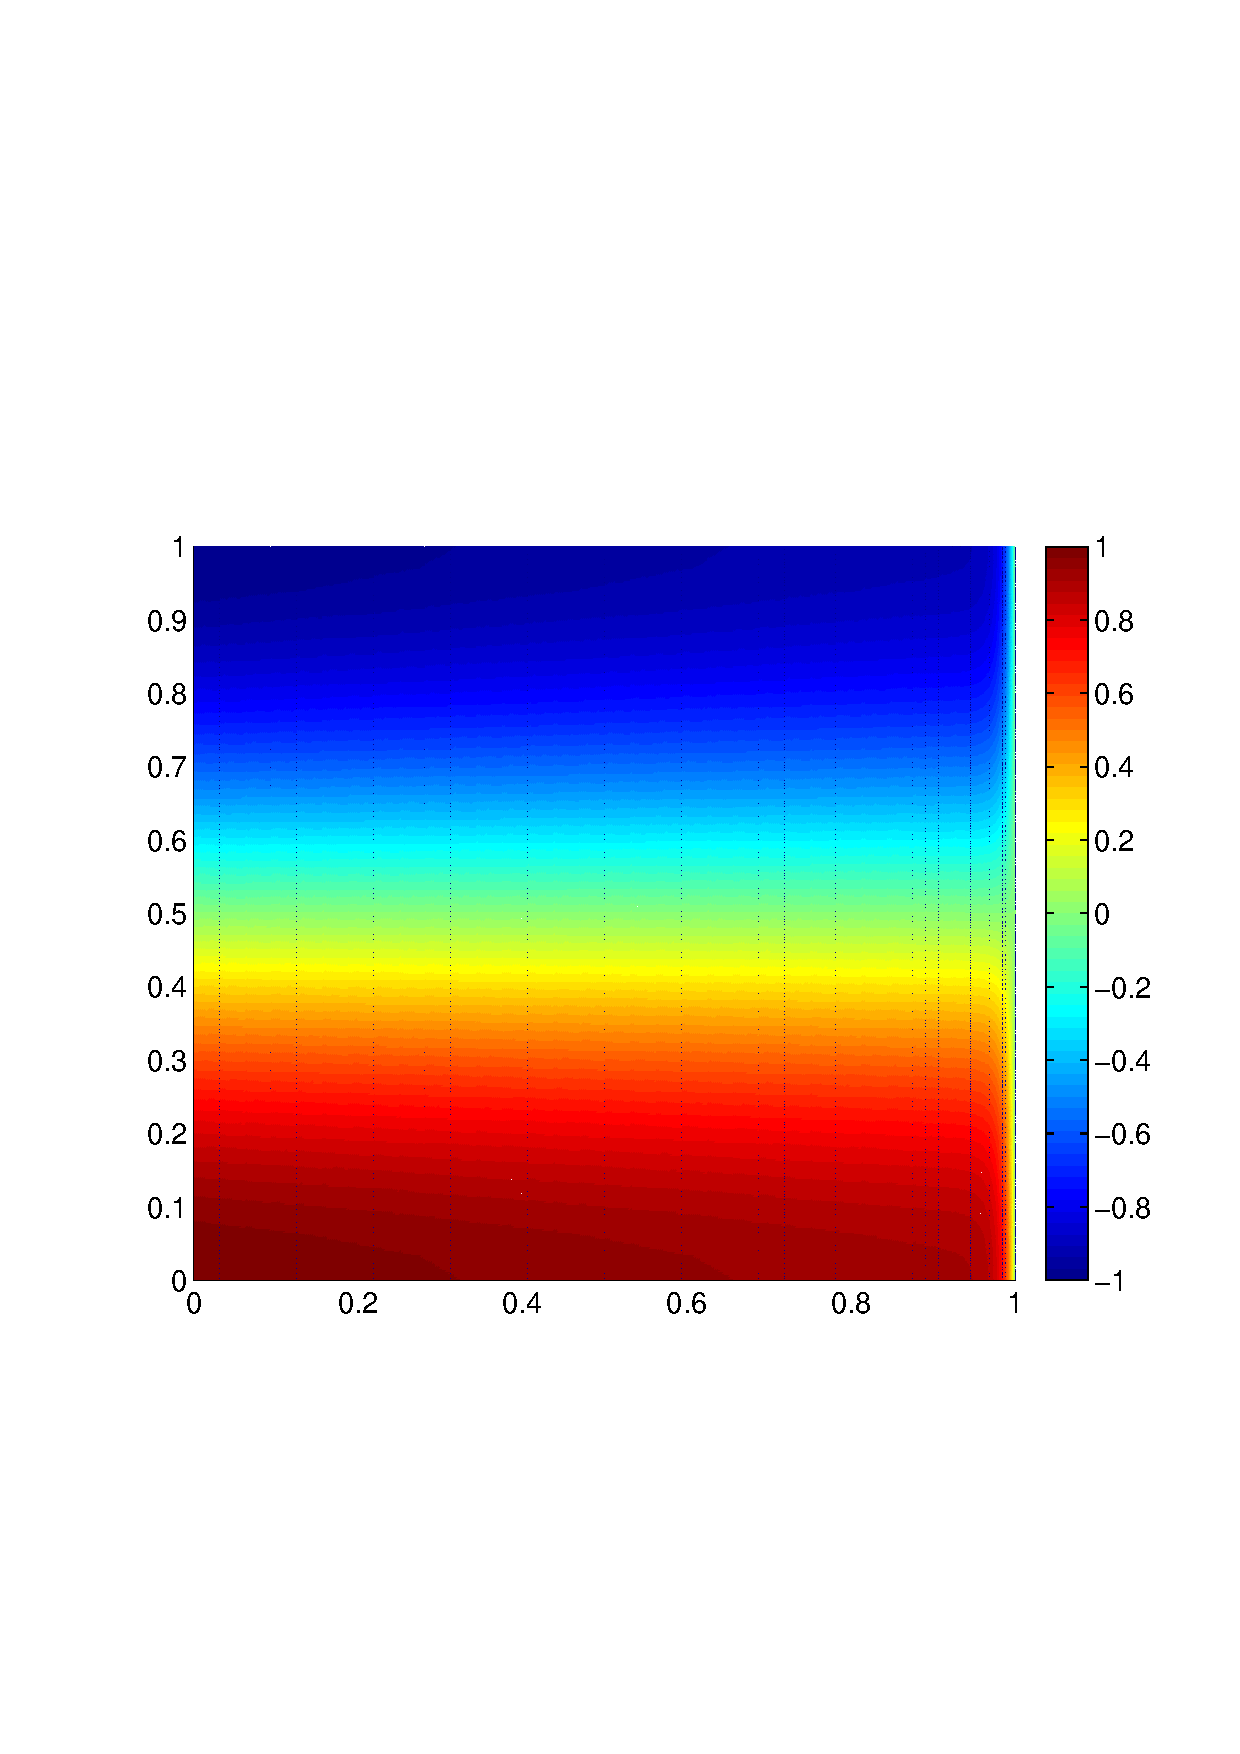
\includegraphics[scale=.37]{figs/wallBC_exact_u.png}
%}
%\subfigure{
%\includegraphics[scale=.37]{figs/wallBC_exact_sigx.png}
%}
%\subfigure{
%\includegraphics[scale=.37]{figs/wallBC_exact_sigy.png}
%}
%\caption{Solution for $u$, $\sigma_x$, and $\sigma_y$ for $\epsilon = .01$, $C_1 = 1$, $C_n=0$, $n\neq 1$}
%\end{figure}

All computations have been done using the adaptive DPG code Camellia, built on the Sandia toolbox Trilinos \cite{Camellia}.

Cite mesh idea of Schwab and Suri \cite{SchwabBoundaryLayers}.  The mesh will consist of two elements, one of width $C\epsilon(p+\del p)$, where $C = O(1)$.  Simpler to implement than Shishkin sub-meshes, which are harder to work with than simple $\del p$ enrichment (submeshes require transformations, assembly, etc).  
\begin{figure}[!h]
\centering
\subfigure{\includegraphics[width=5.7cm]{figs/schwabSuriMesh.pdf}}
\subfigure{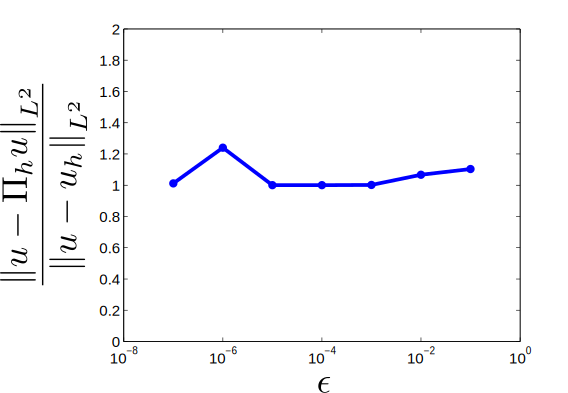
\includegraphics[width=9cm]{figs/schwabSuriResults.pdf}}
\caption{Two-element mesh of Schwab and Suri, tailored to predict boundary layers in conforming test functions, and corresponding ratio of $L^2$ errors for the $L^2$-projected exact solution and the DPG solution, ranging over $\epsilon = 1e-1$ to $\epsilon = 1e-7$ with $C=2$. 
}
\label{fig:schwabSuriMesh}
\end{figure}

At $\epsilon = 1e-6$, there is significant roundoff error in the thin element due to conditioning of highly anisotropic (aspect ratio = $\epsilon^{-1} = 1e6$) and high order elements.  Nevertheless, the solution looks like the $L^2$ solution away from that element.  

\textcolor{red}{Todo: test limiting the aspect ratio to see if you can resolve decently for $\epsilon = 1e-6, 1e-7$.  Try adaptivity as well, and try to explain that $\nor{e}_V$ is far from the actual $L^2$ error due to resolution of test functions but not error rep functions.}

\subsection{Adaptivity with/without boundary layer resolution.}

\subsection{Under-resolution of boundary layers}
We note that globally optimal test functions only produce boundary layers at the global inflow boundary.

\textcolor{red}{Can we quantify the effect of under-resolving boundary layers?}

\begin{align*}
b\LRp{\LRp{u,\sigma, \uh,\fnh},\LRp{v,\tau}} = \LRp{u, \Grad_h\cdot \tau - \beta\cdot \Grad_h v}_{\Oh} + \LRp{\sigma, \frac{1}{\epsilon}\tau + \Grad_h v}_{\Oh} + \LRa{\uh,\tau_n}_{\Gh} + \LRa{\fnh,v}_{\Gh}
\end{align*}
Let $\boldsymbol U$ denote the trial variables $\{u,\sigma, \uh, \fnh\}$. For robustness in $u$, we can choose for $\LRp{v,\tau}$ the conforming solution to the adjoint equation such that 
\begin{align*}
\div \tau - \beta \cdot \grad v &= u \\
\frac{1}{\epsilon} \tau - \grad v &= 0. 
\end{align*}
By doing so, we recover the $L^2$ norm of $u$ from the bilinear form, such that
\[
\nor{u}^2_{L^2(\Omega)} = b\LRp{{\boldsymbol U},\LRp{v,\tau}} = \frac{b\LRp{{\boldsymbol U},\LRp{v,\tau}}}{\nor{\LRp{v,\tau}}_V} \nor{\LRp{v,\tau}}_V \leq \nor{\boldsymbol U}_E \nor{\LRp{v,\tau}}_V
\]
Let $\lesssim$ denote a robust bound in $\epsilon$
\footnote{A bound $a \lesssim b$ is considered robust in some parameter $\epsilon$ if $a \leq C b$ for some constant $C$ independent of $\epsilon$.}
  - if $\nor{\LRp{v,\tau}}_V \lesssim \|u\|_{L^2(\Omega)}$, then we have that
\[
\nor{u}_{L^2(\Omega)} \lesssim \nor{\boldsymbol U}_E
\]
In other words, a necessary condition for a robust method is that the test norm measures global solutions to the adjoint equations in a robust manner.  

The above logic was presented in \cite{DPGrobustness, ChanHeuerBui-ThanhDemkowicz12} in order to motivate necessary conditions with which to construct a test norm for convection-diffusion problems.  However, the same logic can be applied at the discrete level for approximate test functions.  

Include plots of underresolved test functions - show that the inflow boundary layer ``releases" for underresolved approximations.

%If we assume that an underresolved test function behaves similarly to a test function under a larger viscosity, we expect that the term $\nor{\div \tau - \beta \cdot \grad v}_{L^2}$ still remains relatively bounded uniformly in $\epsilon$. However, the term $\nor{\frac{1}{\epsilon}\tau + \grad v}_{L^2}$ does not - analytical calculations in 1D show that this term grows with the Peclet number in the element at the inflow, where the adjoint solution develops a boundary layer. As the boundedness of this term determines the robustness of $\sigma$, our energy norm is
%\begin{align*}
%\nor{\boldsymbol U}_E &\coloneqq \sup_{\LRp{v,\tau}}\LRp{\frac{\LRp{u,\Grad_h \cdot \tau - \beta \cdot \Grad_h v}_{\Omega}}{\nor{\LRp{v,\tau}}_V} + \frac{\LRp{\sigma, \frac{1}{\epsilon}\tau + \Grad_h v}_{\Omega}}{\nor{\LRp{v,\tau}}_V} + \frac{\LRa{\fnh,v}_{\Gamma} - \LRa{\uh,\tau_n}_{\Gamma}}{\nor{\LRp{v,\tau}}_V}} \\
%&\approx \nor{u}_{L^2} + F(\text{Pe})\nor{\sigma}_{L^2} + \nor{\LRp{\uh,\fnh}}
%\end{align*}
%where $F(\text{Pe})$ is some non-decreasing function of the Peclet number. Numerical experiments confirm that, for the quasi-optimal test norm, underresolution of the inflow boundary layer negatively affects mainly the robustness of $u$. 

\subsection{A modification of the adjoint problem}

Modification of adjoint problem: \cite{ChanHeuerBui-ThanhDemkowicz12}.
\begin{itemize}
\item $\nor{\cdot}_{V_{\rm inflow}}$ ??
\end{itemize}


\section{Conclusions}

\begin{itemize}
\item There are three levels at which you should look - the continuous level (the adjoint problem for $L^2$ robustness), the global level (which links the adjoint equation to the test functions), and the localized test norm (which relates local test functions to global test functions). 
\item Your test norm may induce boundary layers even when they're not necessary for adjoint $L^2$ stability.
\item If your test norm promises global boundary layers (that affect robustness), not approximating them leads to a loss of robustness. 
\end{itemize}

You have to account for the boundary layer/$\epsilon$ diffusion scale somehow - either by 
\begin{itemize}
\item adjusting the test norm to account for robustness (weighted test norm), which pushes the $\epsilon$ into the inflow area, 
\item removing the continuous adjoint problem (``convection'' inflow boundary condition), which removes the boundary layer for $L^2$ stability altogether, 
\item resolving the global boundary layers (demonstrated here and in Antii's Shishkin meshes)
\end{itemize}

\section{Acknowledgements}

\textcolor{red}{Thanks to John Evans for several helpful discussions.}

\bibliographystyle{plain}
\bibliography{paper}

\section{Outline}

\begin{enumerate}
\item \textbf{Introduce DPG}
\item \textbf{Globally optimal test space}: Introduce globally optimal testing, give proof of weakly-conforming global test space contained in localized test space. Make note of the jumps being approximated by the flux/trace space and note that this poses difficulty for different singular perturbation problems like wave propagation.
\begin{itemize}
\item Relate globally optimal test functions back to $L^2$ optimal global test functions.  
\end{itemize}
\item \textbf{Discuss application to convection-diffusion}: describe issue of resolution of local test functions and the presence of boundary layers that appear on elements that aren't in globally optimal test functions.  Define \textit{robustness}.
\begin{itemize}
\item Discuss the different boundary layers - boundary layers in \textit{local/global DPG test functions}, and boundary layers in \textit{$L^2$ optimal test functions}.
\item There are two cases: If the $L^2$-optimal test functions produce boundary layers, they must be dealt with
\begin{itemize}
\item Test norm - weight the test norm such that it doesn't behave non-robustly in the boundary layer area (give graph test norm example as well)
\item Discrete approximation - approximate test functions such that they resolve the boundary layer robustly.  
\end{itemize}
If the $L^2$-optimal test functions do not produce boundary layers, the story then depends on your test norm.
\begin{itemize}
\item Test norm - can use a test norm that doesn't produce BL test functions, i.e. remove the weight.
\item Discrete approx - if you use the graph test norm, boundary layers are still produced.
\end{itemize}
\end{itemize}
\item \textbf{Numerical experiments}: (energy/$L^2$ error and their ratio as resolution of inflow layer increases), 
\begin{itemize}
\item Mention effects of underresolution of boundary layers with the new inflow condition/graph test norm, as well as the robust test norm (i.e. underresolution of boundary layer in $v$).  Plot 5 global optimal test functions each - 1 for u, 2 for sigma, 2 fluxes (streamline/cross-stream), 
\begin{itemize} 
\item Graph norm 
\item Weighted norm
\item Unweighted norm
\end{itemize}
\end{itemize}
\item \textbf{Conclusions}: The behavior of DPG really depends on two things for convection-diffusion: if your discrete test functions are approximated such that they are (globally) robust in your test norm, and if your test norm measures the $L^2$ optimal test functions in a robustly continuous manner.  

\end{enumerate}

\end{document}

%\subsection{The strong form of the trial-to-test operator}
%
%Under the graph test norm 
%\[
%\LRp{v,\delta v}_{V(K)} = \LRp{A_h^*v,A_h^*\delta v}_{L^2(K)} + (v,\delta v)_{L^2(K)},
%\]
%element-local test functions are induced as solutions of 
%\[
%\LRp{v,\delta v}_{V(K)} = (u,A_h^*\delta v)_K + \LRa{\uh,\delta v}_{\partial K}
%\]
%Under proper regularity assumptions, this variational problem corresponds to the strong problem
%\begin{align*}
%A_hA_h^*v + v &= A_hu, \quad \text{on $K$}\\
%\gamma\LRp{A_h^*v} &= \uh.
%\end{align*}
